% Preamble
\documentclass[12pt]{report} % Defines the report document class with 12pt font size.
\usepackage[utf8]{inputenc} % Allows the use of UTF-8 characters in the document.
\usepackage[T1]{fontenc} % Enhances font encoding for European and extended character sets.
\usepackage{graphicx} % Enables the inclusion and manipulation of graphics.
\usepackage{listings} % Provides source code listings.
\usepackage{amsmath} % Provides support for mathematical equations.
\usepackage{float} % Provides additional options for figure placement such as H.
\usepackage{hyperref} % Adds hyperlink capabilities to the document.
\usepackage[nameinlink,noabbrev]{cleveref} % Provides support for clever references.
\usepackage{chapterbib} % Provides support for multiple bibliographies in the document.
\usepackage{lmodern} % Provides the Latin Modern font family.
\usepackage[top=1in]{geometry} % Adjust the top margin
\usepackage{fancyhdr} % Provides support for custom headers and footers.
\usepackage[numbers]{natbib} %  Provides support for author-year citations. 
%\usepackage{sloppy}
% Usse CTAN to download the package and install it in your LaTeX distribution.


% Custom styling
\usepackage{styles/mystyle} % Loads defined custom styles.

% Document begins here
\begin{document}


% Title page simple
% \title{Title of the Document}
% \author{Author}
% \date{\today}
% \maketitle
% Title page with custom styling

\begin{titlepage}
    \centering
    \vspace*{1cm}
    
    \Huge
    \textbf{Deep Learning Architectures}
    
    \vspace{0.5cm}
    \LARGE
    A Comprehensive Overview and Guide
    
    \vspace{1.5cm}
    
    \textbf{Your Name}
    
    \vfill
    
    This document presents a detailed exploration \\
    of various deep learning architectures, \\
    their implementations, and applications. \\
    The Document was written using ChatGPT.
    
    \vspace{0.8cm}
    
    \Large
    FH JOANNEUM GmbH\\
    System Test Engineering\\
    Graz\\
    \today
    
    \vspace{2cm}
    
    
\includegraphics[width=0.4\textwidth]{figures/logo_fhj_stm.jpg}
    
    \vspace{3cm}
\end{titlepage}


% Abstract
\begin{abstract}
This is the abstract of the document, providing a summary of the contents.
\end{abstract}

% Table of Contents
\tableofcontents
\newpage

% Include chapters
\chapter{Contents}
\label{chap:contents}

This is a content

\section{section}
A section.
\subsection{subsection}
A subsection.

\section{Text}\label{sec:text}
This section is meant to show how to integrate text structured in section ans subsactions can be add to the document.

\subsection{Various Formatting Styles in Text}\label{subsec:formatting_styles_text}
Here is an example text that demonstrates various formatting styles:

\begin{itemize}
    \item \textbf{Bold text}
    \item \textit{Italic text}
    \item \underline{Underlined text}
    \item \texttt{Code text}
\end{itemize}

You can use these formatting styles to enhance the visual appearance of your text in your LaTeX document.

\section{Image Section}
\label{image_section}

% Section title slide
\sectiontitleframe{Image Section}

\begin{frame}{Image with Caption}
  \begin{figure}
    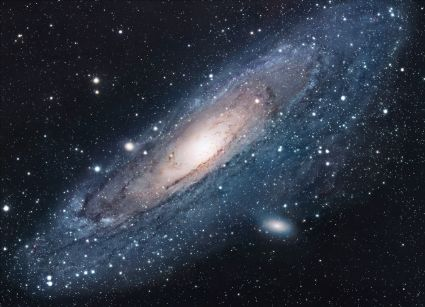
\includegraphics[width=0.7\textwidth]{figures/universe.jpg} % Replace 'example-image' with your image file
    \caption{This is a beautiful image.}
    \label{fig:sampleimage}
  \end{figure}
\end{frame}

\begin{frame}{Reference to the Image}
  In the previous frame, we saw a beautiful image (see Figure~\ref{fig:sampleimage}). It reminds us of the importance of visuals in our presentations.
\end{frame}
\newpage

\section{Table}\label{sec:table}
This section is meant to show how to integrate tables in the document.

\newcolumntype{M}{>{\centering\arraybackslash}p{0.7cm}}

\begin{table}[ht]
\centering
\begin{spacing}{1.1}\caption{Sample Table One}\label{table:tableOne}
\scriptsize
\begin{tabular}{|p{3.75cm}|M|M|M|M|M|M|M|M|M|M|}
\multicolumn{1}{c|}{\bf{}} &
\multicolumn{5}{c|}{\cellcolor{black!10}\bf{Gross-Pitch Error (GPE) (\%)}}  &
\multicolumn{5}{c|}{\cellcolor{black!10}\bf{Fine-Pitch Error (FPE) (Hz)}} \\
\hline
{GPE/FPE input signal} & \multicolumn{5}{c|}{{SNR (dB)}}  &
\multicolumn{5}{c|}{{SNR (dB)}} \\ \cline{2-6} \cline{7-11}
{} & {-6} & {-3} & {0} & {3} & {6} & {-6} & {-3} & {0} & {3} & {6} \\ \hline
{(UB): est. BM ({PEFAC})} & 26.07 & 23.67 & 21.10 & 19.41 & 18.56 & 0.71 & 0.59
& 0.75 & 0.63 & 0.69\\ \hline
{(UB): est. RM ({PEFAC})} & 25.16 & 22.29 & 18.51 & 18.62 & 16.54 & 0.71 & 0.63
& 0.79 & 0.74 & 0.88\\ \hline \hline
{est. BM ({PEFAC})} & 48.01 & 39.75 & 32.13 & 28.22 & 23.26 & 1.49 & 0.84
& 0.86 & 0.92 & 0.69\\ \hline
{est. BM ({proposed PE})} & 39.37 & 33.77 & 27.96 & 25.05 & 21.90 & 1.25 &
0.85 & 0.80 & 0.87 & 0.88\\ \hline
{est. RM ({PEFAC})} & 52.45 & 44.44 & 37.80 & 31.98 & 27.65 & 1.99 &
1.09 & 1.26 & 0.89 & 0.85\\ \hline
{est. RM ({proposed PE})} & 46.32 & 39.21 & 32.13 & 28.89 & 25.34 & 1.46 &
0.97 & 0.94 & 0.83 & 0.69\\ \hline \hline
{(LB): Mixed signal ({PEFAC})} & 66.2 & 60.55 & 53.98 & 46.52 & 40.33 & 2.96 & 2.42 & 2.22
& 1.71 & 1.46\\ \hline

\end{tabular}
\end{spacing}
\end{table}

\subsection{Reference to Table}\label{subsec:reference_table}
\noindent The Table of above is referenced here \cref{table:tableOne}.

\section{Mathematical Formula}
\label{sec:math-formula}

This section demonstrates how to include a mathematical formula in your LaTeX document. For instance, consider the quadratic formula:

\begin{equation}
\label{eq:quadratic}
x = \frac{-b \pm \sqrt{b^2 - 4ac}}{2a}
\end{equation}

You can reference this formula elsewhere in the document using the label 'eq:quadratic'.

\newpage
\section{Python Code Section}
\label{python_code_section}
\sectiontitleframe{Python Code Section}

\begin{frame}[fragile]{Python Code Listing}
    \begin{lstlisting}[caption={Sample Python Code}, label=lst:pythoncode]
  from (*@\module{sklearn.preprocessing}@*) import (*@\class{PolynomialFeatures}@*)
 
  # This is a comment in Python
  def say_hello(name):
      print(f"Hello, {name}!")
  
  say_hello("world")
    \end{lstlisting}
  \end{frame}
  
  \begin{frame}{Reference to the Python Code}
    The Python function in Listing~\ref{lst:pythoncode} demonstrates a simple greeting.
  \end{frame}
  
\section{List Examples}

\subsection{Unnumbered List}
Here is an unnumbered list:
\begin{itemize}
    \item First item
    \item Second item
    \item Third item
\end{itemize}

\subsection{Numbered List}
And here is a numbered list:
\begin{enumerate}
    \item First item
    \item Second item
    \item Third item
\end{enumerate}
\chapter{references}
\label{chap:refereces}

After \cref{chap:contents} we come to chapter references.

\section{To Text}
\label{sec:to_text} % Unique label used for referencing the section in other parts of the document.

Here some text that references the \cref{sec:text}.

\section{To Image}
\label{sec:to_image} % Unique label used for referencing the section in other parts of the document.

Here the reference to the \cref{fig:image1}.

\section{To Table}
\label{sec:to_table} % Unique label used for referencing the section in other parts of the document.

Here the reference to  \cref{tab:my_table}.

\section{To Math Formula}
\label{sec:to_math_formula} % Unique label used for referencing this section

This section demonstrates how to reference a equation within the document, like \cref{eq:quadratic}.

\section{To Python Code}
\label{sec:to_python_code} % Unique label used for referencing the section in other parts of the document.

Here the reference to the \cref{lst:python_code}.

\section{citations}
\label{sec:citations}
Here is a section with references to a book \citep{exampleBook}, a journal article \citep{exampleArticle}, a website \citep{exampleWebsite}, and a conference paper \citep{examplePaper}.




% Bibliography
\newpage
\bibliography{bibliography/references}

% Appendices
\appendix
\chapter*{Appendix A}
\addcontentsline{toc}{chapter}{Appendix A}

This is Appendix A. You can include additional details, extended analysis, or supplementary data here. Appendices are useful for providing extra information without cluttering the main body of the document.

\chapter*{Appendix B}
\addcontentsline{toc}{chapter}{Appendix B}

Appendix B could include extended tables, additional figures, or raw data relevant to your document. This section allows you to present all relevant material that supports your work but is too extensive to include in the main chapters.


% End of the document
\end{document}

